\documentclass[compress,red]{beamer}
\usepackage[utf8]{inputenc}
\usepackage{pgf}
\usepackage{ucs}
\usepackage{amsmath}
\usepackage{amsfonts}
\usepackage{amssymb}
\usepackage[russian]{babel}
\usepackage{graphicx}
\usepackage{wrapfig}

\mode<presentation>

\usetheme{Warsaw}

\definecolor{Red}{rgb}{1,0,0}
\definecolor{Blue}{rgb}{0,0,1}
\definecolor{Green}{rgb}{0,1,0}
\definecolor{magenta}{rgb}{1,0,.6}
\definecolor{lightblue}{rgb}{0,.5,1}
\definecolor{lightpurple}{rgb}{.6,.4,1}
\definecolor{gold}{rgb}{.6,.5,0}
\definecolor{orange}{rgb}{1,0.4,0}
\definecolor{hotpink}{rgb}{1,0,0.5}
\definecolor{newcolor2}{rgb}{.5,.3,.5}
\definecolor{newcolor}{rgb}{0,.3,1}
\definecolor{newcolor3}{rgb}{1,0,.35}
\definecolor{darkgreen1}{rgb}{0, .35, 0}
\definecolor{darkgreen}{rgb}{0, .6, 0}
\definecolor{darkred}{rgb}{.75,0,0}

\xdefinecolor{olive}{cmyk}{0.64,0,0.95,0.4}
\xdefinecolor{purpleish}{cmyk}{0.75,0.75,0,0}

\useoutertheme[subsection=false]{smoothbars}

\title{Что такое ``облачные технологии''}
\author{Информатика}
\date{}
%\usecolortheme{dolphin}

\begin{document}
%%титульная страница
\maketitle
%% основные моменты

\section{Облака}

\begin{frame}[fragile]
  \frametitle{Рост технологий}
  \centerline{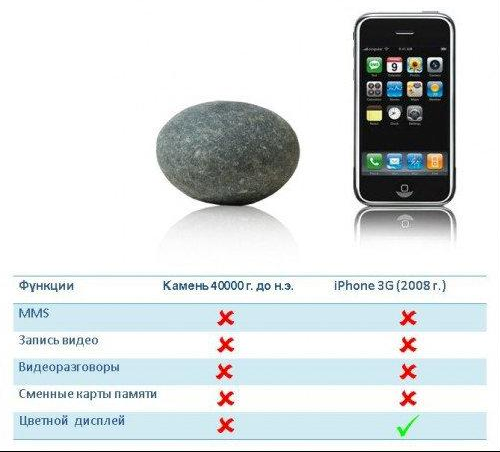
\includegraphics[width=0.6\textwidth]{images/iphone-vs-stone.png}}
\end{frame}

\begin{frame}[fragile]
  \frametitle{Облачные сервисы}
  \centerline{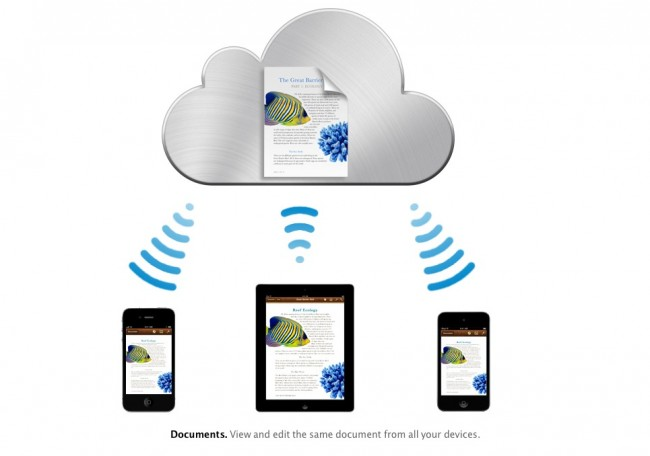
\includegraphics[width=0.9\textwidth]{images/icloud.jpg}}
\end{frame}

\subsection{Что такое облако}
\begin{frame}[fragile]
  \frametitle{Что такое облако?}
  \begin{itemize}
    \item Облако --- группа компьютеров, на которых пользователи хранят свои данные.
    \item Разделяют \emph{облачные хранилища данных} и \emph{облачные вычисления}.
    \item Во втором случае компьютеры облака используются для обработки больших массивов данных и/или сложных вычислений.
  \end{itemize}
\end{frame}

\subsection{Saas}
\begin{frame}
  \begin{center}
    \Huge{SaaS}
  \end{center}
  \begin{center}
    \Large{Software as a service}
  \end{center}
\end{frame}

\subsection{Свойства Saas}
\begin{frame}[fragile]
  \frametitle{Модель SaaS}
  \begin{itemize}
    \item Приложение возможно использовать удалённо.
    \item Оплата в зависимости от использования.
    \item Нет отдельной платы за техническое обслуживание.
    \item Нет необходимости глобальных инвестиций в программное обеспечение.
    \item Быстрота внедрения, ясность и предсказуемость, мультиплатформенность.
  \end{itemize}
\end{frame}

\subsection{Примеры SaaS}
\begin{frame}[fragile]
  \frametitle{SaaS}
  \centerline{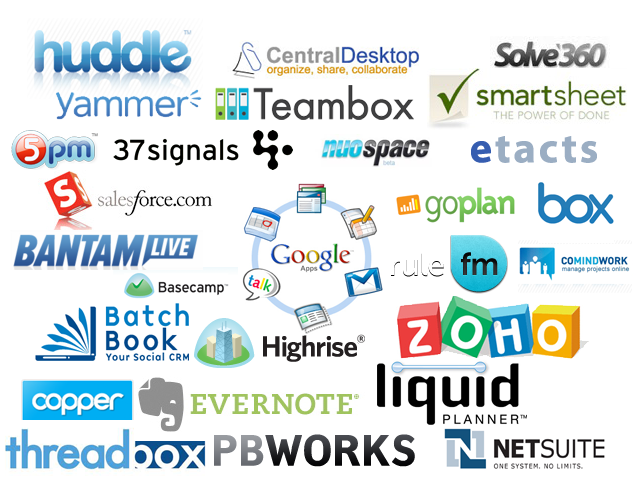
\includegraphics[width=0.8\textwidth]{images/saas.png}}
\end{frame}

\subsection{В чём минусы}
\begin{frame}
  \begin{center}
    \Huge{В чём минусы облачных технологий?}
  \end{center}
\end{frame}


\section{Хранилища данных}
\subsection{Use case 1}
\begin{frame}
  \begin{center}
    \Huge{Use case 1}
  \end{center}
  \begin{center}
    \Large{Домашний~компьютер и рабочий~компьютер}
  \end{center}
\end{frame}

\subsection{Use case 2}
\begin{frame}
  \begin{center}
    \Huge{Use case 2}
  \end{center}
  \begin{center}
    \Large{Папка для совместной работы}
  \end{center}
\end{frame}

\subsection{Use case 3}
\begin{frame}
  \begin{center}
    \Huge{Use case 3}
  \end{center}
  \begin{center}
    \Large{Публикация файлов в Сети}
  \end{center}
\end{frame}

\section{Облачные хранилища}

\subsection{Уже используем}
\begin{frame}
  \begin{center}
    \Huge{Уже используем}
  \end{center}
  \begin{center}
    \Large{Google Drive}
  \end{center}
\end{frame}

\subsection{Встречайте Dropbox}
\begin{frame}[fragile]
  \frametitle{Встречайте Dropbox}
  \centerline{
\includegraphics[width=0.7\textwidth]{images/dropbox-icon.png}}
\end{frame}

\subsection{Встречайте Dropbox 2}
\begin{frame}[fragile]
  \frametitle{Встречайте Dropbox}
  \centerline{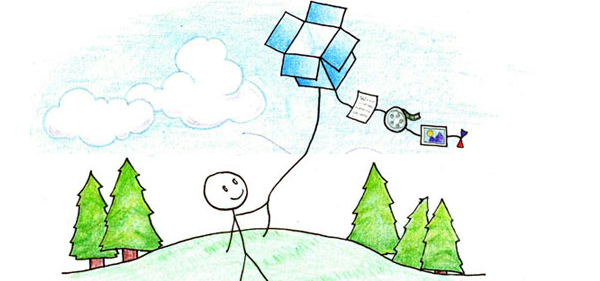
\includegraphics[width=1.0\textwidth]{images/ilovedropbox1.jpg}}
\end{frame}

\subsection{Встречайте Dropbox 3}
\begin{frame}[fragile]
  \frametitle{Встречайте Dropbox}
  \centerline{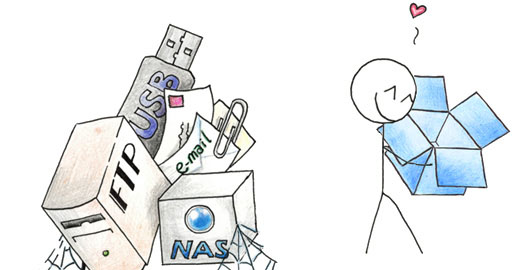
\includegraphics[width=1.0\textwidth]{images/ilovedropbox2.jpg}}
\end{frame}

\subsection{Описание}
\begin{frame}[fragile]
  \frametitle{Dropbox}
  \begin{itemize}
    \item Dropbox позволяет просто и легко синхронизировать данные между различными устройствами, а также опубликовывать их в Интернете.
    \item Он делает это незаметно и в фоновом режиме, позволяя пользователю сконцентрироваться на действительно важных задач и не думать о ПО.
    \item Любыми материалами можно поделиться с другом. Можно даже сделать папки совместными, когда любые изменения у одного человека в общей папке практически мгновенно появляются у другого.
    \item Есть программы под Windows, Linux, OS X.
    \item Первая ``доза'' --- бесплатно (2 Гб + бонусы).
  \end{itemize}
\end{frame}

\section{Dropbox}
\subsection{Dropbox 1}
\begin{frame}[fragile]
  \frametitle{Описание Dropbox}
  \centerline{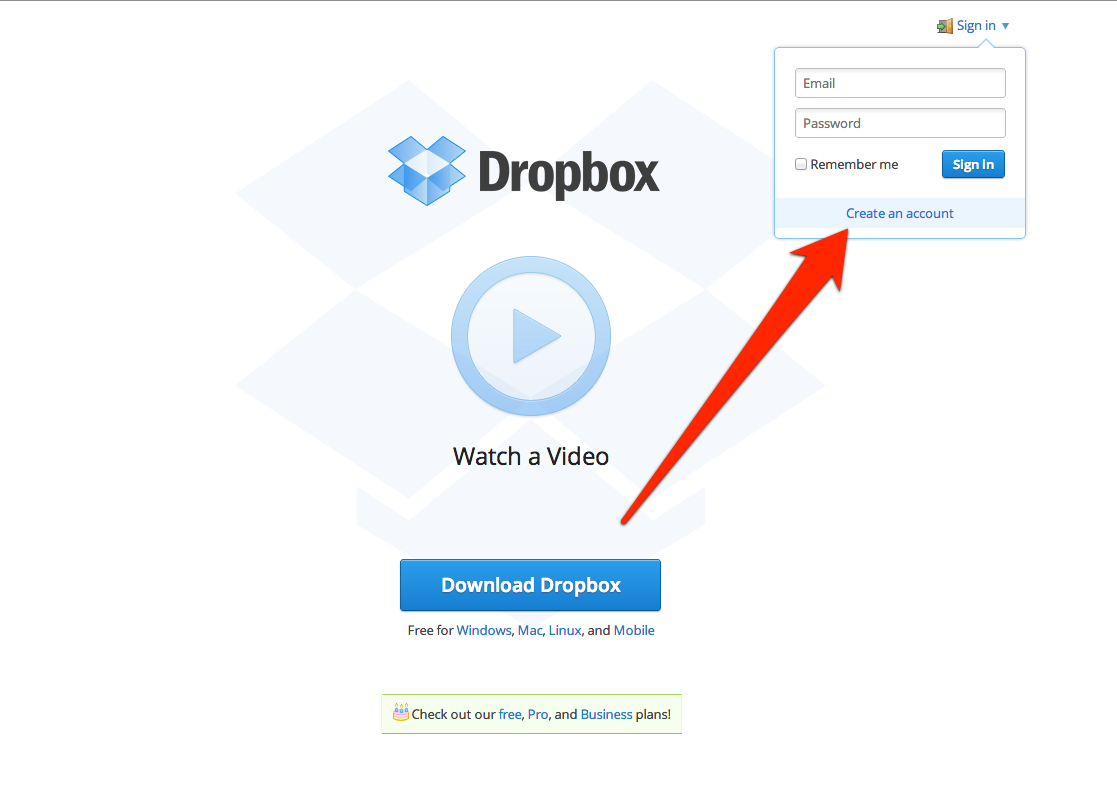
\includegraphics[width=0.9\textwidth]{images/dropbox1.png}}
\end{frame}

\subsection{Dropbox 2}
\begin{frame}[fragile]
  \frametitle{Описание Dropbox}
  \centerline{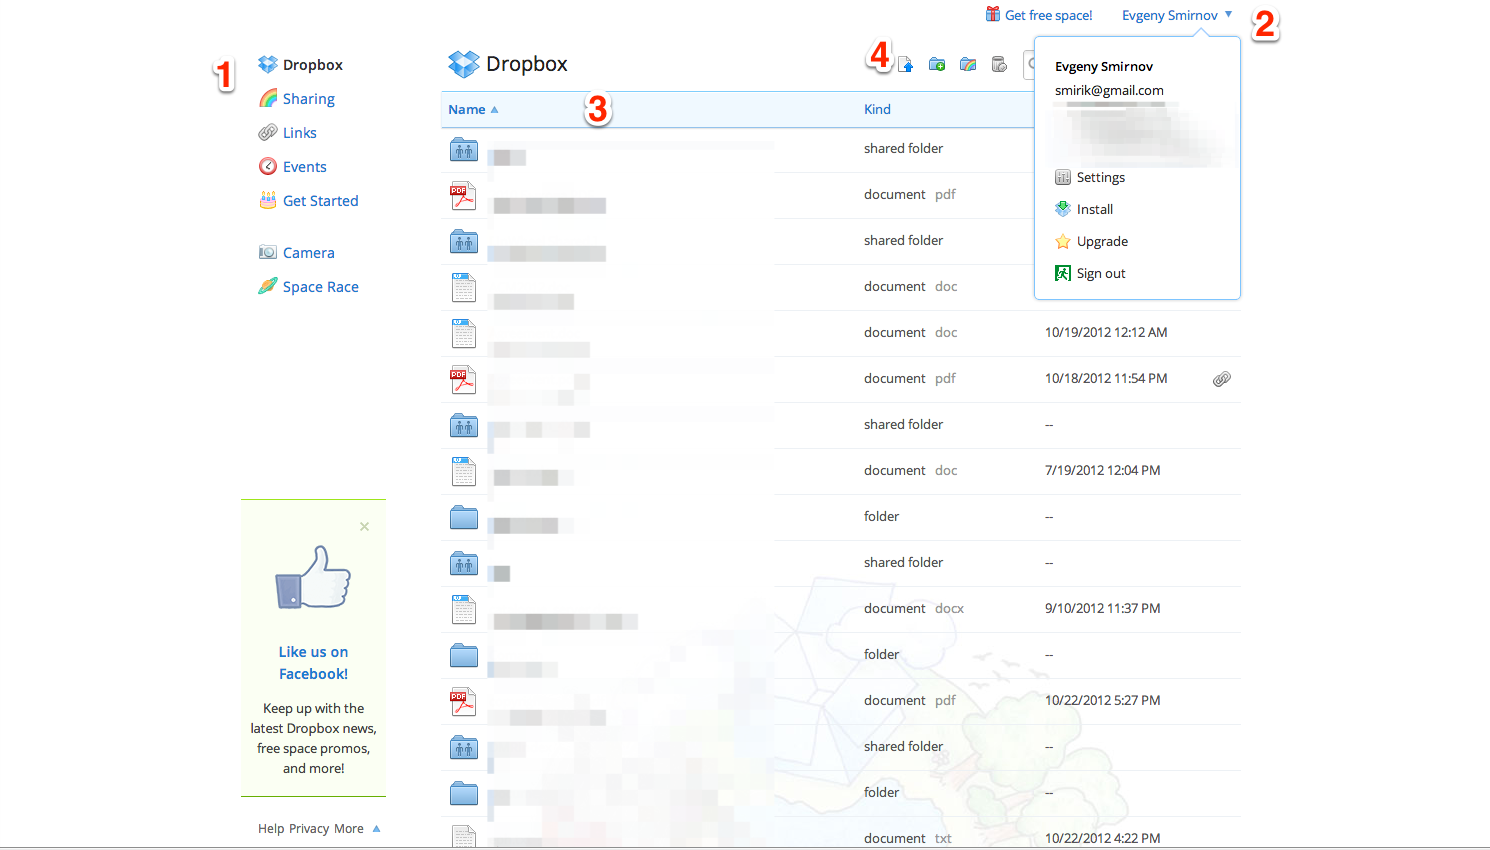
\includegraphics[width=0.9\textwidth]{images/dropbox2.png}}
\end{frame}

\subsection{Dropbox 3}
\begin{frame}[fragile]
  \frametitle{Описание Dropbox}
  \centerline{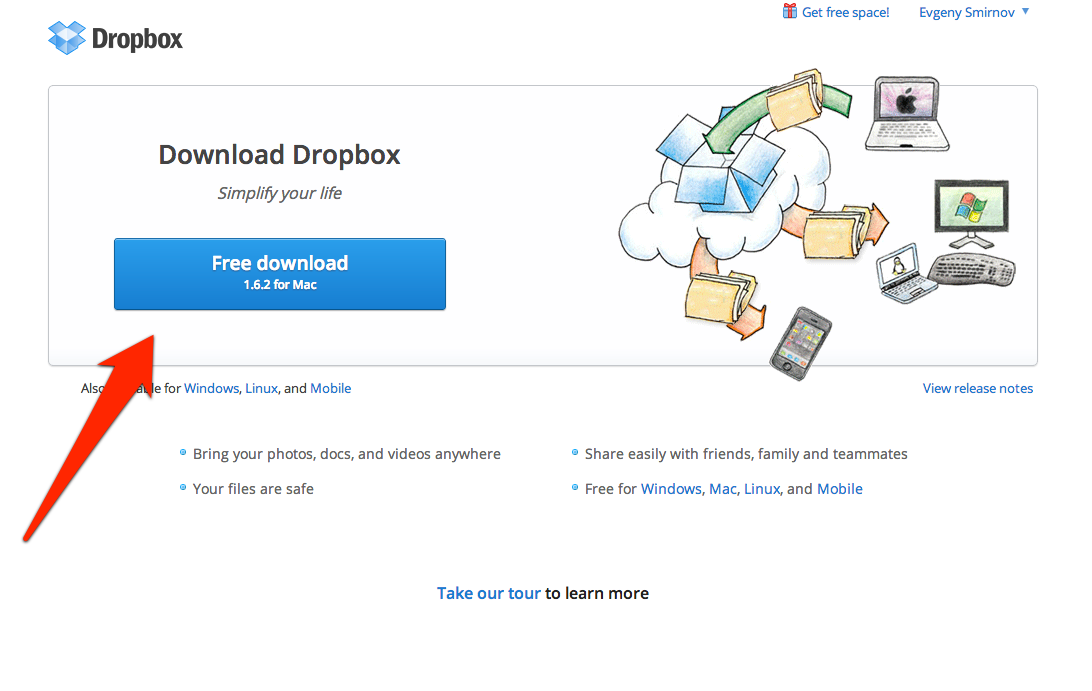
\includegraphics[width=0.9\textwidth]{images/dropbox3.png}}
\end{frame}

\subsection{Ссылка}
\begin{frame}
  \begin{center}
    \Huge{http://dropbox.com}
  \end{center}
  \begin{center}
    \Huge{http://db.tt/d2RyFKa}
    
    \small{реферальная ссылка,~+500~Мб}
  \end{center}
\end{frame}

\end{document}